\documentclass[a4paper,12pt,oneside,pdflatex,italian,final,twocolumn]{article}

\usepackage[utf8]{inputenc}
\usepackage{parallel}
\usepackage{siunitx}
\usepackage{booktabs}
\usepackage{fancyhdr}
\usepackage{subcaption}
\usepackage{listings}
\usepackage{hyperref}
\usepackage{pdfpages}

\usepackage[export]{adjustbox}
\usepackage[margin=0.5in]{geometry}
\addtolength{\topmargin}{0in}

\usepackage{libertine}
\renewcommand*\familydefault{\sfdefault}
\usepackage[T1]{fontenc}

\urlstyle{sf}
\hypersetup{
	colorlinks=true, %set true if you want colored links
	linktoc=all,     %set to all if you want both sections and subsections linked
	linkcolor=blue,  %choose some color if you want links to stand out
	urlcolor=blue,   %url color
}

\title{Portable Bluetooth Stetoscope}
\author{Achmadi ST MT}
\date{Desember 2022}

\begin{document}
	
	\pagestyle{fancy}
	
	\lhead{VibrasticLab}
	\chead{\today}
	\rhead{Specification Document v1.0}
	
	\onecolumn
	
	\begin{figure}
		
	\end{figure}\begin{minipage}{0.47\textwidth}
		\centering
		
	\end{minipage}
	\hfill
	\begin{minipage}{0.47\textwidth}
		\raggedleft
		\Huge \textbf{Portable Bluetooth Stetoscope}
	\end{minipage}

	\section{Overview}
	
	\begin{itemize}
		\item Fowarding Audio from I2S Microphone (based on INMP441) to any A2DP Compatible Audio Sink.
		
		\item Provides spesific frequency capture using 3D printed stetoscope head
		
		\item Battery operated using embedded system approach using ESP32 as the core
		
		\item The design currently in very early stage and not for end usage
		
	\end{itemize}
	
	\raggedright
	\section{MockUp 3D}
	
	Mock up 3D of the prototype without outer case (except stetoscope head)
	
	\centering
	\begin{figure}[!ht]
		\centering
		\includegraphics[width=\textwidth,]{images/steto_overview.png}
		\caption{Prototype Unit}
	\end{figure}

	\raggedright
	\section{PCB Design}

	Current PCB Schematic and Layout Design
	
	\newpage
	\includepdf[pages=-,angle=-90]{pdf/esp32steto_sch.pdf}
	
	\newpage
	\includepdf[pages=-,angle=-90]{pdf/esp32steto_pcb.pdf}
	
	\newpage
	\includepdf[pages=-,angle=180]{pdf/esp32steto_bom.pdf}
	
	\newpage
	\section{Project Repositories}
	
	List of Project Repositories:
	\begin{itemize}
		\item KiCAD Circuit Design: \\
		\url{https://github.com/VibrasticLab/ehealth-iot/tree/master/esp32-steto/circuit}
		
		\item ESP-IDF Firmware Draft: \\
		\url{https://github.com/VibrasticLab/ehealth-iot/tree/master/esp32-mic-a2dp}
		
		\item Stetoscope Open Design: \\
		\url{https://github.com/GliaX/Stethoscope}
	\end{itemize}
	
	\section{Electronic Unit Cost Estimation}
	
	\begin{tabular}{|l|l|l|}
		\toprule
		Item & Price-Qty & URL \\
		\midrule
		ESP32 WROOM 32 & Rp. 47.900 & \href{https://www.tokopedia.com/altrosurabaya/esp-wroom-32-esp32-wifi-bt-ble-mcu-module-only-smd-smt}{Tokopedia} \\
		AMS117-3v3 & Rp 1.200 & \href{https://www.tokopedia.com/radioshop/ams117-ams117-3-3v-ams117-3v3-ams117-3-3-smd-regulator-chipset}{Tokopedia} \\
		Mic INMP441 & Rp. 42.000 & \href{https://www.tokopedia.com/easyware-id/inmp441-omnidirectional-microphone-module-mems-i2s-interface}{Tokopedia} \\
		LCD OLED SSD1306 & Rp. 33.000 & \href{https://www.tokopedia.com/easyware-id/oled-128x64-lcd-i2c-spi-0-96-inch-white-blue-yellow-blue-backlight-i2c-yellow-blue}{Tokopedia} \\
		PCB Prototyping & Rp. 200.000 & \href{https://www.tokopedia.com/geraicerdas/cetak-pcb-1-keping-single-double-layer-rapid-prototyping-satuan}{Tokopedia} \\
		Tombol/LED/Passives & Rp. 200.000 & Pasar Genteng Surabaya \\
		Wire dkk & Rp. 50.000 & Pasar Genteng Surabaya \\
		Ongkir Tokopedia & Rp. 100.000 & - \\
		\midrule
		Total & Rp. 674.100  & - \\
		\bottomrule
	\end{tabular}

	\section{Case/Head Development Estimation}
	
	\begin{tabular}{|l|l|l|}
		\toprule
		Item & Price-Qty & URL \\
		\midrule
		3D Printer Kingroon & Rp. 2.450.000 & \href{https://www.tokopedia.com/3dzaiku/3d-printer-kingroon-kp3s-new-linear-rail-direct-drive-32-bit-tmc2225}{Tokopedia} \\
		Fimalent Material & Rp. 700.000 & \href{https://www.tokopedia.com/3dzaiku/esun-3d-filament-terbaru-silk-pla-1-75-mm}{Tokopedia} \\
		\midrule
		Total & Rp. 3.150.000  & - \\
		\bottomrule
	\end{tabular}

\end{document}

